
The SolKz benchmark \cite{repa87} is similar to the SolCx benchmark.
but the viscosity is now a function of the space coordinates: 
\begin{equation}
\mu(y)=\exp(By) \quad {\rm with} \quad B=13.8155
\end{equation}
It is however not a discontinuous function but grows exponentially with the vertical coordinate so that its overall variation is again $10^6$. 
The forcing is again chosen by imposing a spatially variable density variation as follows:
\begin{equation}
\rho(x,y)=\sin(2y) \cos(3\pi x)
\end{equation}
Free slip boundary conditions are imposed on all sides of the domain.
This benchmark is presented in \cite{zhon96} as well and is studied in \cite{dumg11} and \cite{gemd13}.

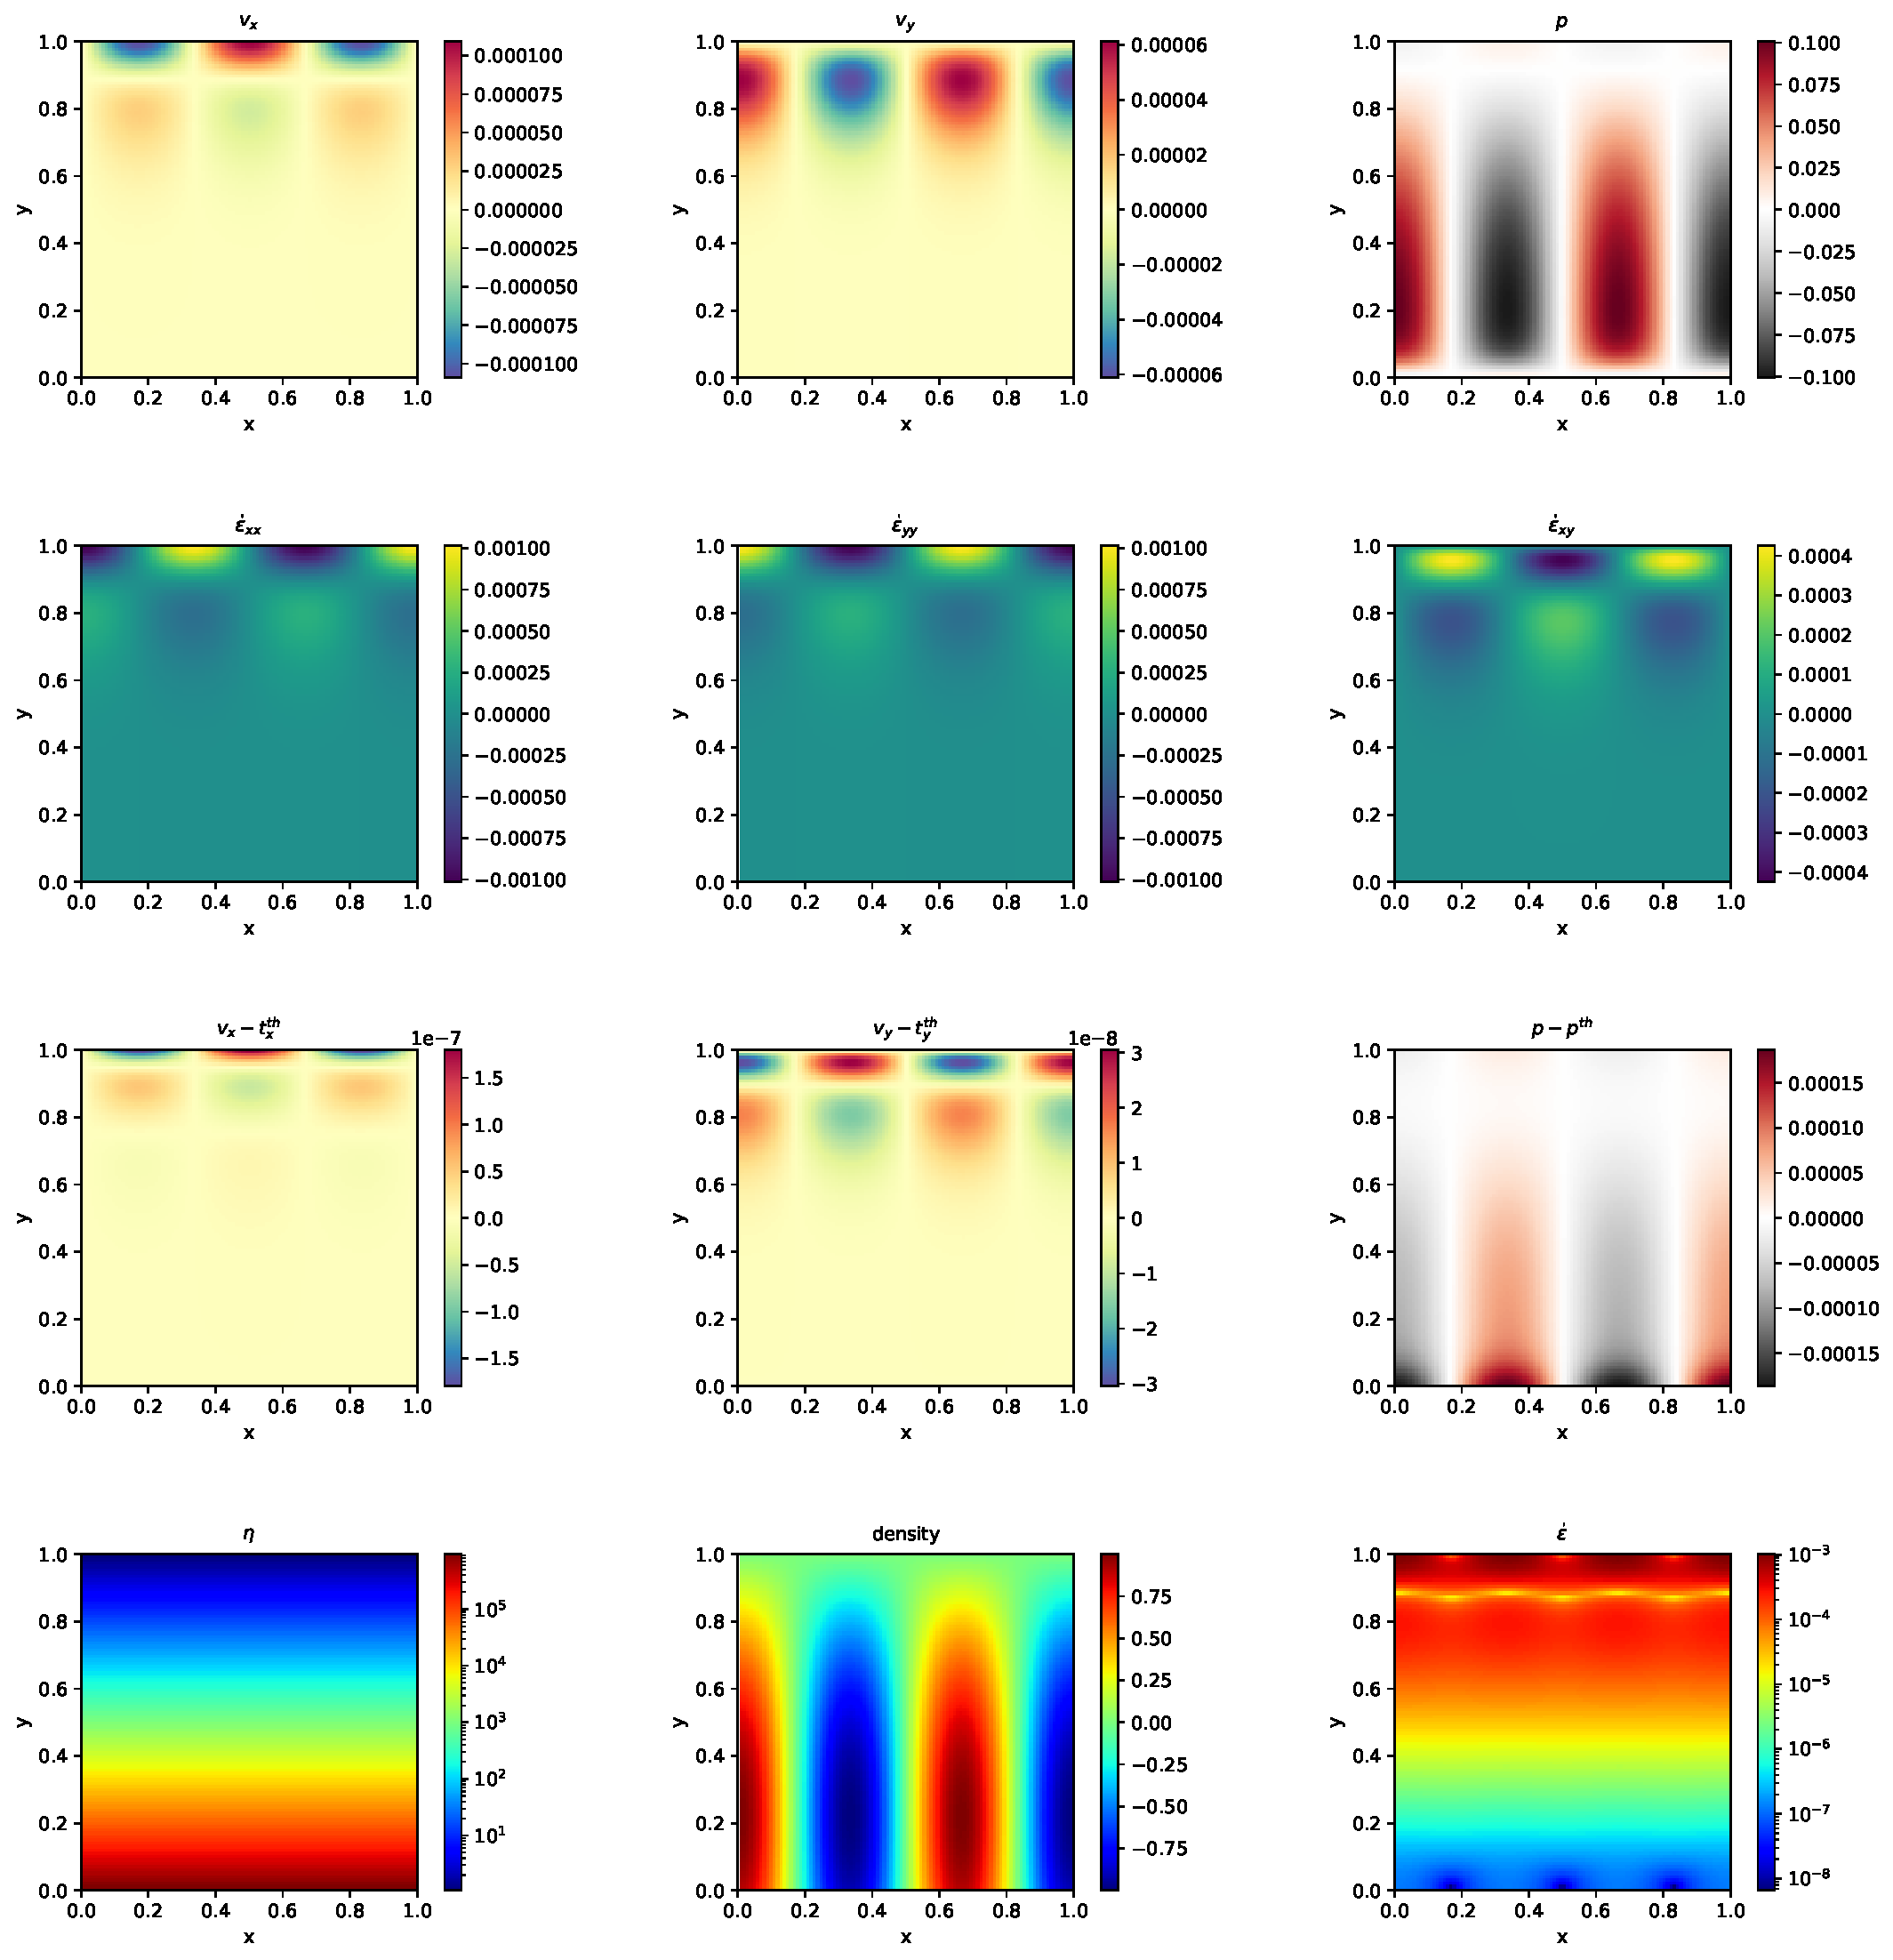
\includegraphics[width=12cm]{python_codes/fieldstone_06/results/solution.pdf}

\begin{center}
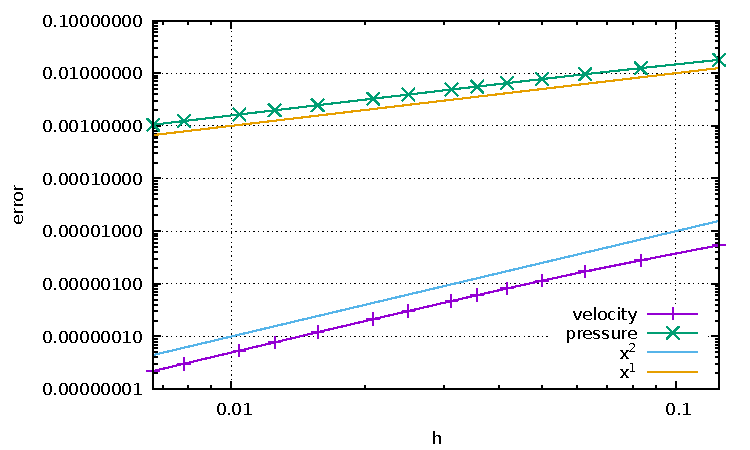
\includegraphics[width=8cm]{python_codes/fieldstone_06/results/errors.pdf}\\
{\captionfont Velocity and pressure error as a function of mesh size.}
\end{center}
